\begin{ReasoningBox}[title=Inductive Reasoning] % 可以通过 title 参数修改标题
    % --- 第一部分：问题描述与图片 ---
    % \begin{minipage}[t]{0.58\textwidth}
    \begin{wrapfigure}{r}{0.3\textwidth}
        \centering
        % wrapfigure 通常顶部会有多余空白，使用负 vspace 向上提，让图片和第一行文字对齐
        \vspace{-20pt} 
        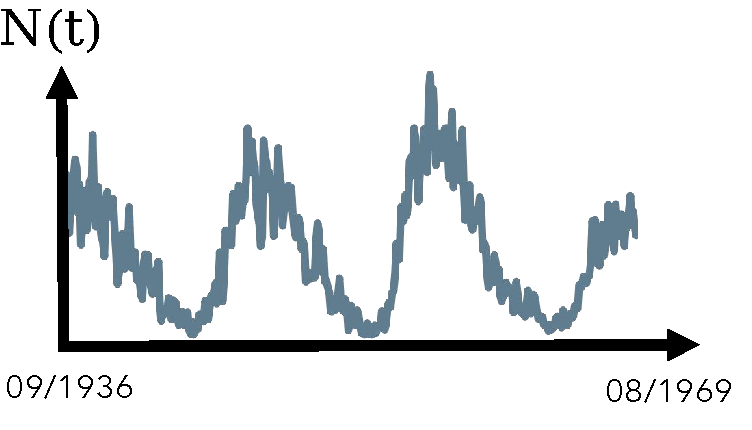
\includegraphics[width=\linewidth]{blocks/sample_cases_success/inductive.pdf}
        % 调整底部的留白
        \vspace{-20pt}
    \end{wrapfigure}
        \textbf{Question:} This historical time series shows the monthly mean number of sunspots---those cooler, dark patches on the Sun's surface caused by intense magnetic activity---from 09/1936 to 08/1969, where each timestamp represents a month. Based on this data, the predicted monthly mean sunspot number for 02/1979 (rounded to the nearest integer) is?

    \vspace{0.5em}

    % --- 第二部分：选项 ---
    \textbf{Answer Choices:} \\ (A) 18 \\ (B) 35 \\ (C) 48 \\ (D) 195 \\ 
    \textbf{Correct Answer:} \textcolor{correctgreen}{(D)} \\
\end{ReasoningBox}